 \section{Кластеризация}
 
Данная задача состоит в разделении точек в пространстве на кластеры близко расположенных.

\subsection{Метрика качества кластеризации}

Как и для задач обучения с учителем, хочется уметь понимать, хорошо ли мы решили задачу - нужно научиться измерять качество кластеризации. 

Так, например, даже не зная число кластеров, можно
перебрать \textit{К} в \textbf{K-Means} и выбрать гиперпараметр с лучшим качеством.

Одним из примеров метрики может быть метрика \textbf{силуэт}.

Для одного элемента $x$ она считается так:

$S(x)=\frac{b(x)-a(x)}{\max (a(x), b(x))}$

$a(x)=$ среднее расстояние от $x$ до точек того же кластера.

$b(x)=$ среднее расстояние от $x$ до точек ближайшего кластера.

Значение \textit{силуэта} для кластера равно среднему значению $S(x)$ от каждого элемента.

Чем он больше тем лучше кластер отделим от других кластеров.

Примеры из выборки можно отсортировать по значению \textit{силуэта} для каждого примера и по
присвоенной метке кластера. Такое представление позволяет отфильтровать шумные примеры (у
которых силуэт меньше некоторого порога).
 
 \subsection{Алгоритм K-Means}
 
Нужно в начале выбрать K центров кластеров (K - гиперпараметр). Далее итеративно выполняются 2 шага, пока обновления не перестанут происходить:
\begin{enumerate}
    \item Обновить кластеры, приписав каждой точке кластер самого близкого к ней центра
    \item Обновить центр каждого кластера как центр масс его точек
\end{enumerate}

\begin{center}
    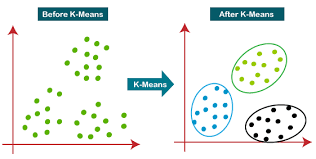
\includegraphics[scale=1]{tickets/pictures/k_means.png}
\end{center}

Плюсы :
\begin{itemize}
    \item простой и понятный
\end{itemize}

Минусы :
\begin{itemize}
    \item нужно знать K
    \item слишком простая модель, кластер = выпуклая околокруглая штука, так как это по сути диаграмма Вороного
    \item если плохо выбрать начальные центры, может сойтись к плохому результату
\end{itemize}

Поэтому обычно K-Means запускают несколько раз и выбирают лучший результат.

\subsection{DBSCAN}

\textbf{DBSCAN} строит столько кластеров, сколько получится, причем многие вершины могут не войти ни в один кластер, они называются выбросами.

\textit{DBSCAN} опирается на два гиперпараметра:

\textit{eps} - означает расстояние, на котором две вершины считаются соседями.
 
\textit{min-samples} - означает сколько нужно соседей из кластера, чтобы считать вершину коренной вершиной кластера.

Сам алгоритм состоит из таких шагов:
\begin{enumerate}
    \item Выбрать соседей для каждой вершины на расстоянии до eps
    \item Найти компоненты связности коренных вершин - добавляем вершину в компоненту коренных, если у нее хотя бы min-samples соседей лежат в этой компоненте
    \item Добавить оставшиеся вершины в самый популярный кластер соседей, если есть соседи
    \item Оставшиеся вершины - это выбросы
\end{enumerate}

\begin{center}
    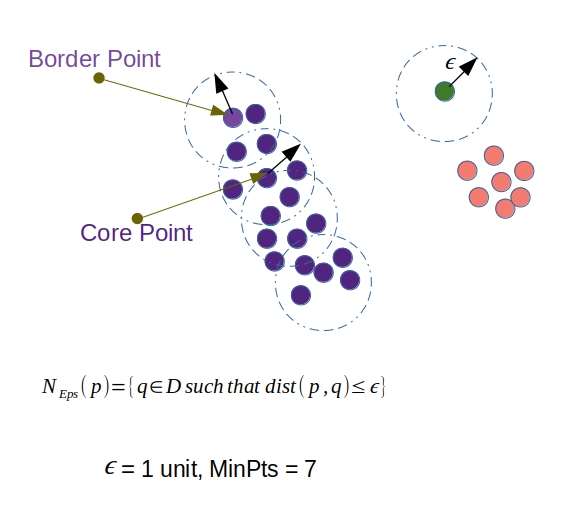
\includegraphics[scale=0.6]{tickets/pictures/dbscan.png}
\end{center}

Плюсы :
\begin{itemize}
    \item сам подберет число кластеров
    \item опирается на плотность точек, кластеры могут быть вытянутыми и даже невыпуклыми
\end{itemize}

Минусы :
\begin{itemize}
    \item нужно подбирать два других параметра
    \item алгоритм считает, что в разных частях данных плотности должны быть примерно одинаковыми
\end{itemize}

\subsection{Агломеративная кластеризация}

Интуиция у алгоритма очень простая:
\begin{enumerate}
    \item Начинаем с того, что высыпаем на каждую точку свой кластер
    \item  Сортируем попарные расстояния между центрами кластеров по возрастанию
    \item  Берём пару ближайших кластеров, склеиваем их в один и пересчитываем центр кластера
    \item  Повторяем п. 2 и 3 до тех пор, пока все данные не склеятся в один кластер
\end{enumerate}
Чтобы найти пару ближайших кластеров берут не только расстояние между центрами, бывают и такие метрики:
\begin{itemize}
    \item Single linkage — минимум попарных расстояний между точками из двух кластеров
    \item Complete linkage — максимум попарных расстояний между точками из двух кластеров
    \item Average linkage — среднее попарных расстояний между точками из двух кластеров
    \item Centroid linkage — расстояние между центроидами двух кластеров
\end{itemize}

\begin{center}
    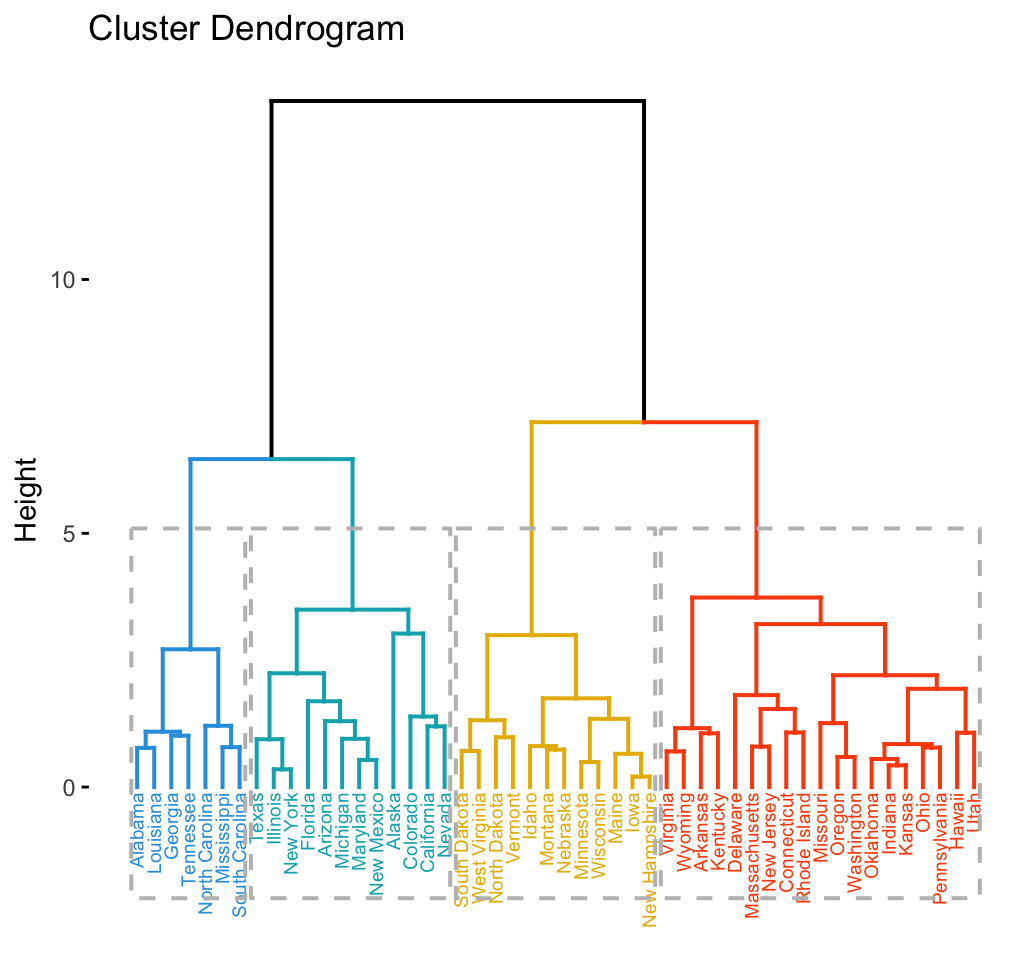
\includegraphics[scale=0.3]{tickets/pictures/agg_clus.jpg}
\end{center}

По итогам выполнения такого алгоритма строится дерево склеивания кластеров. Глядя на него можно определить, на каком этапе оптимальнее всего остановить алгоритм.